\documentclass[../Bachelorarbeit.tex]{subfiles}
\begin{document}

\section*{Anhang} \label{anhang}
\addcontentsline{toc}{section}{Anhang}
Dieser Abschnitt der Arbeit beinhaltet sämtliche Anhänge, die nicht im Hauptteil eingebunden wurden.\\
Anschließend findet sich der komplette Stromlaufplan des Systems. Wichtig zu beachten ist, dass der Stand des Stromlaufplanes in dieser Arbeit zum Zeitpunkt des Lesens vermutlich veraltet ist, da Erweiterungen \bzw Änderungen an der Laboranlage vorgenommen wurden. An aktueller Stromlaufplan muss folglich nachgereicht werden.\\
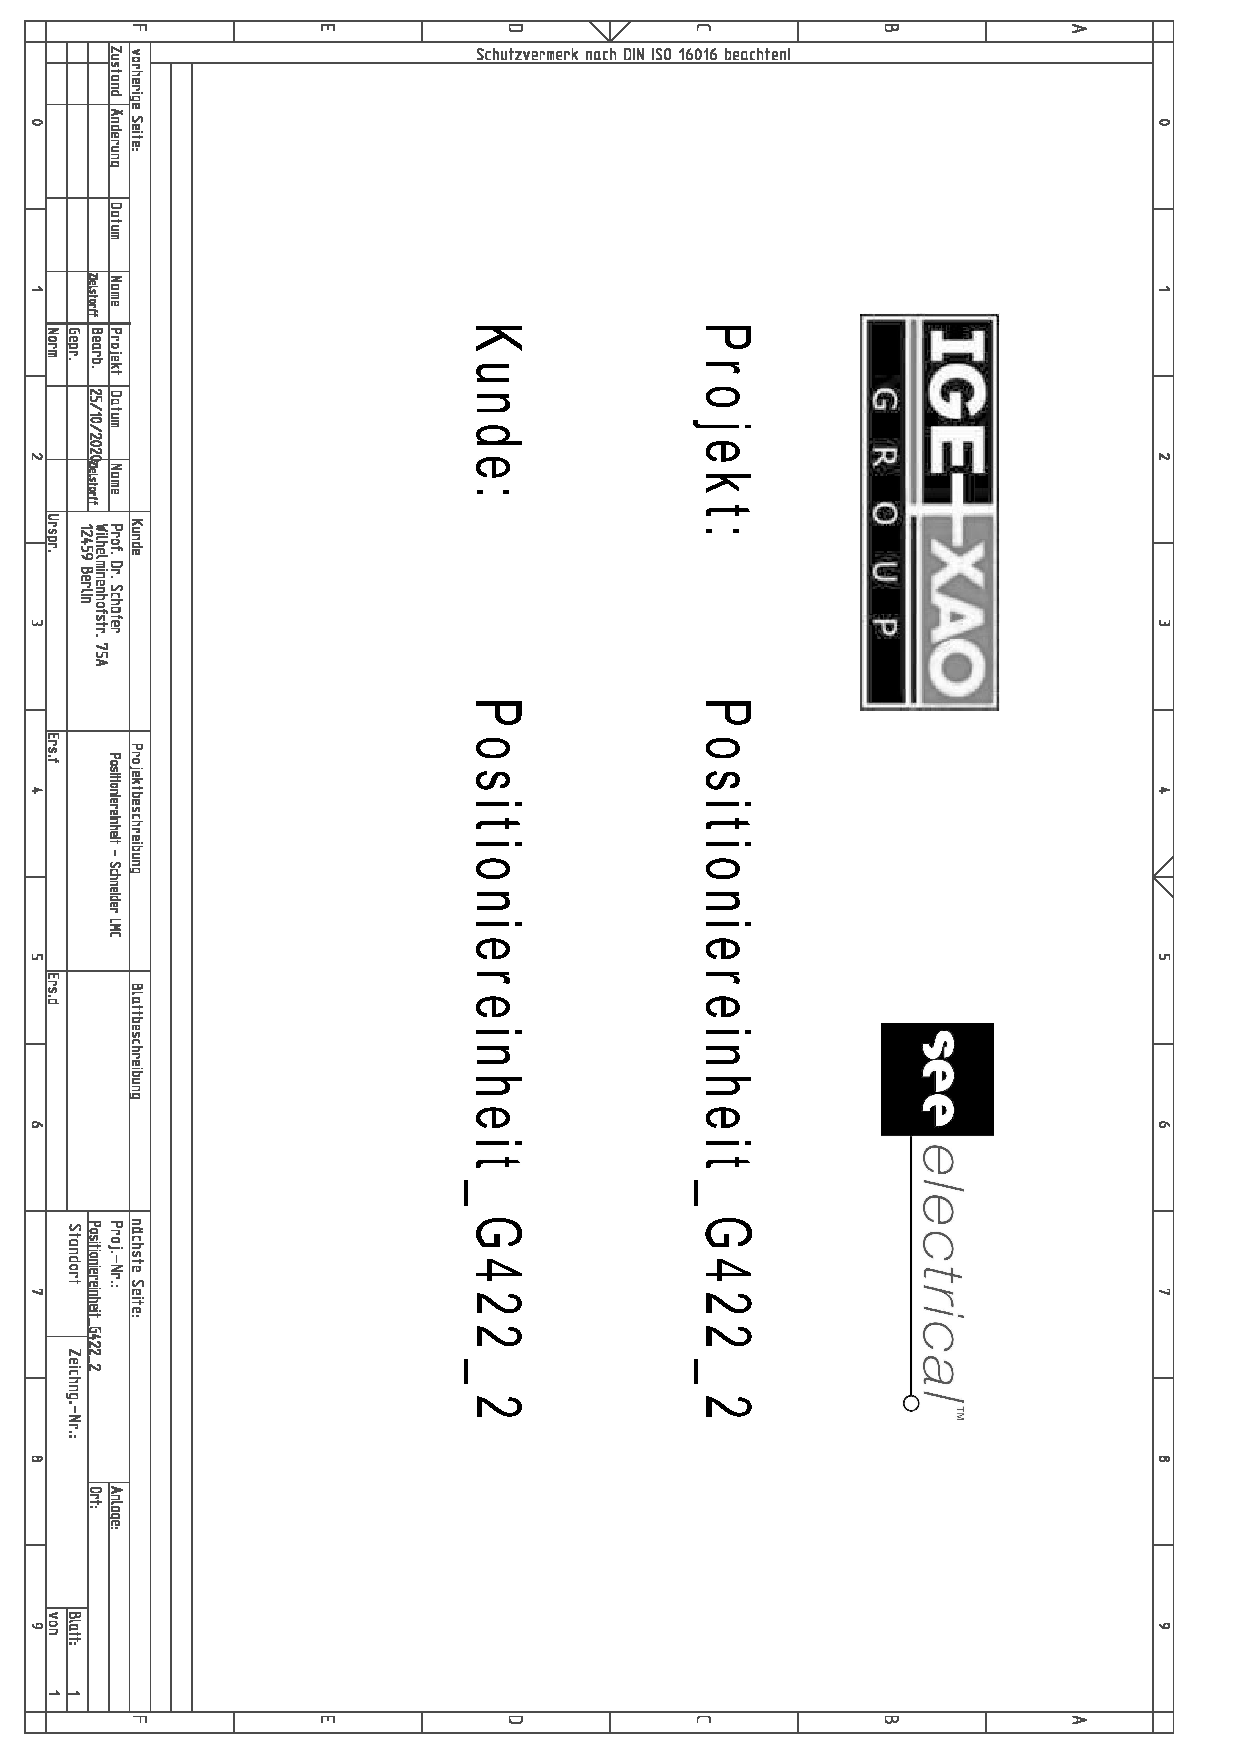
\includepdf{Images/slp1.pdf}
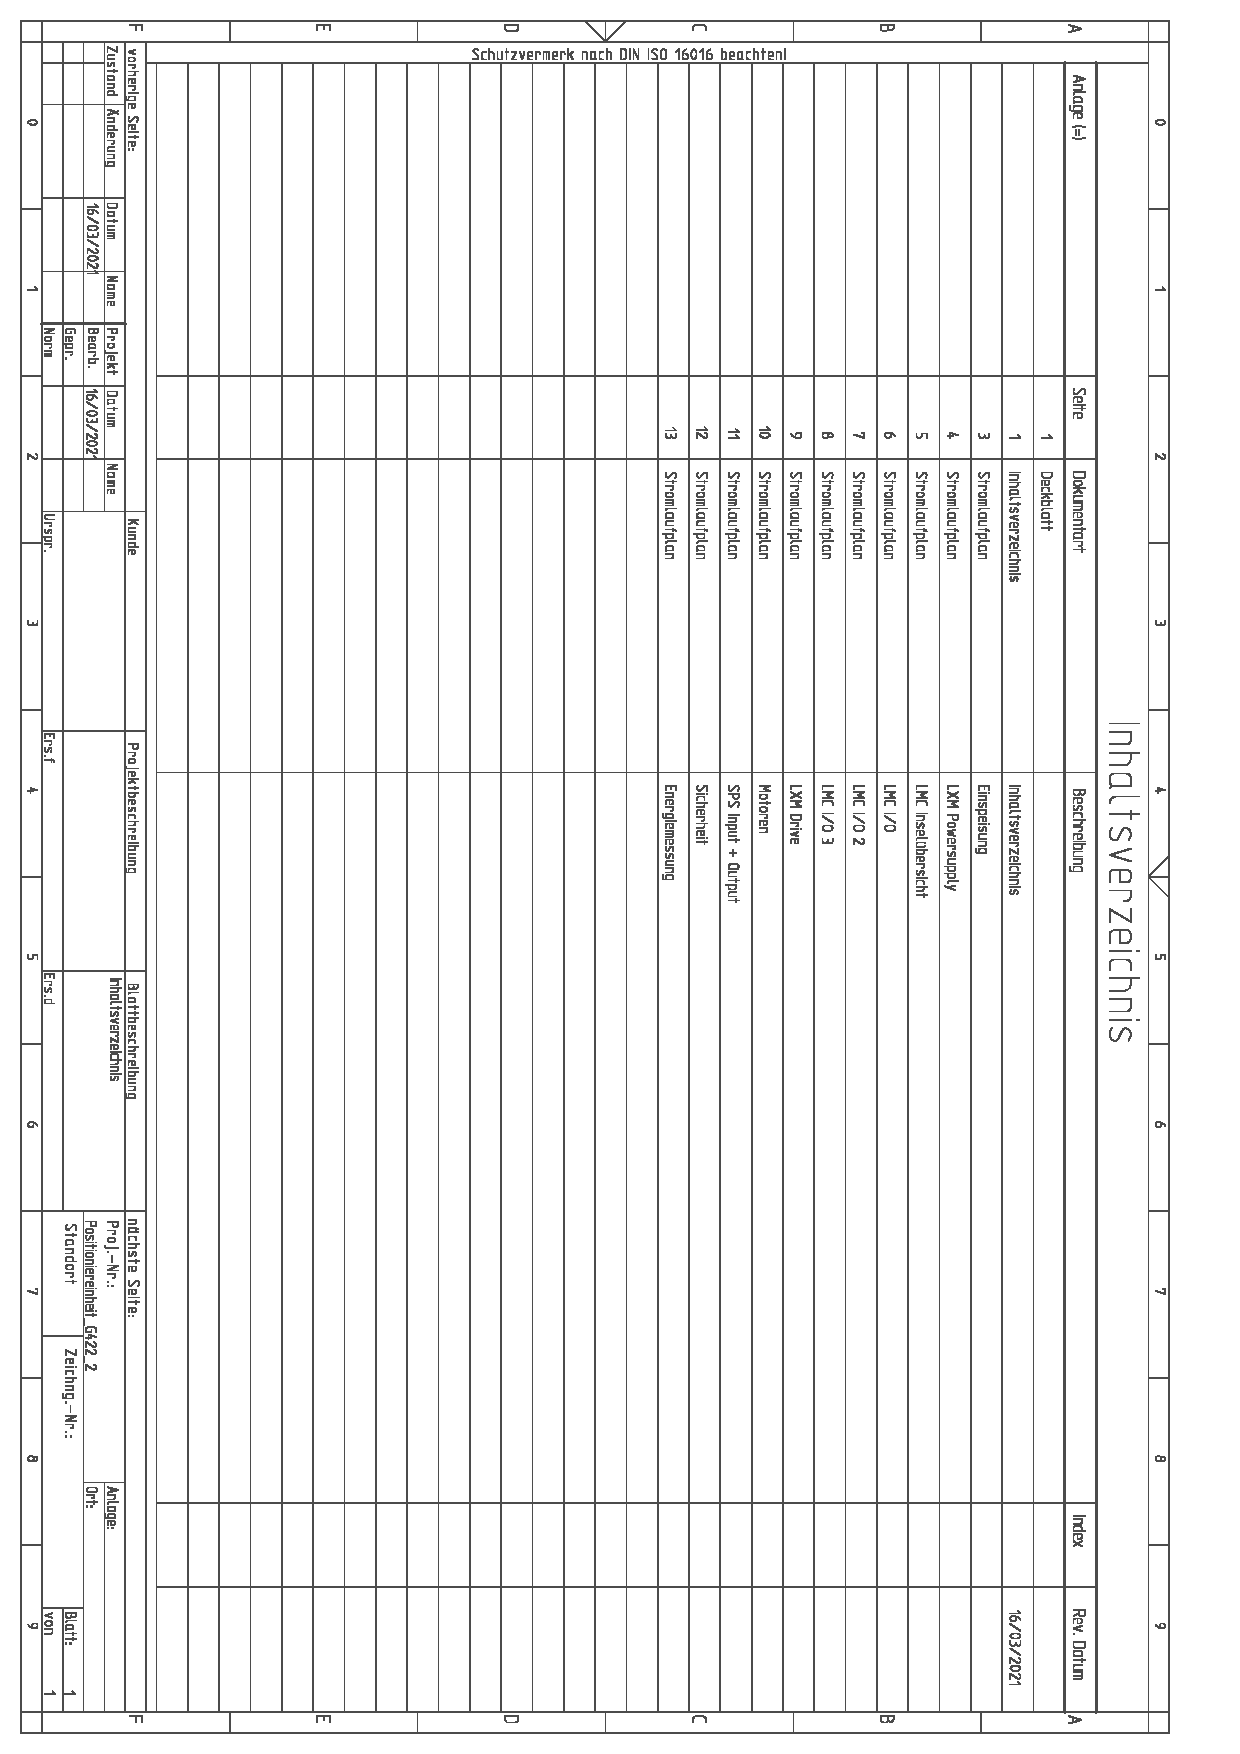
\includepdf{Images/slp2.pdf}
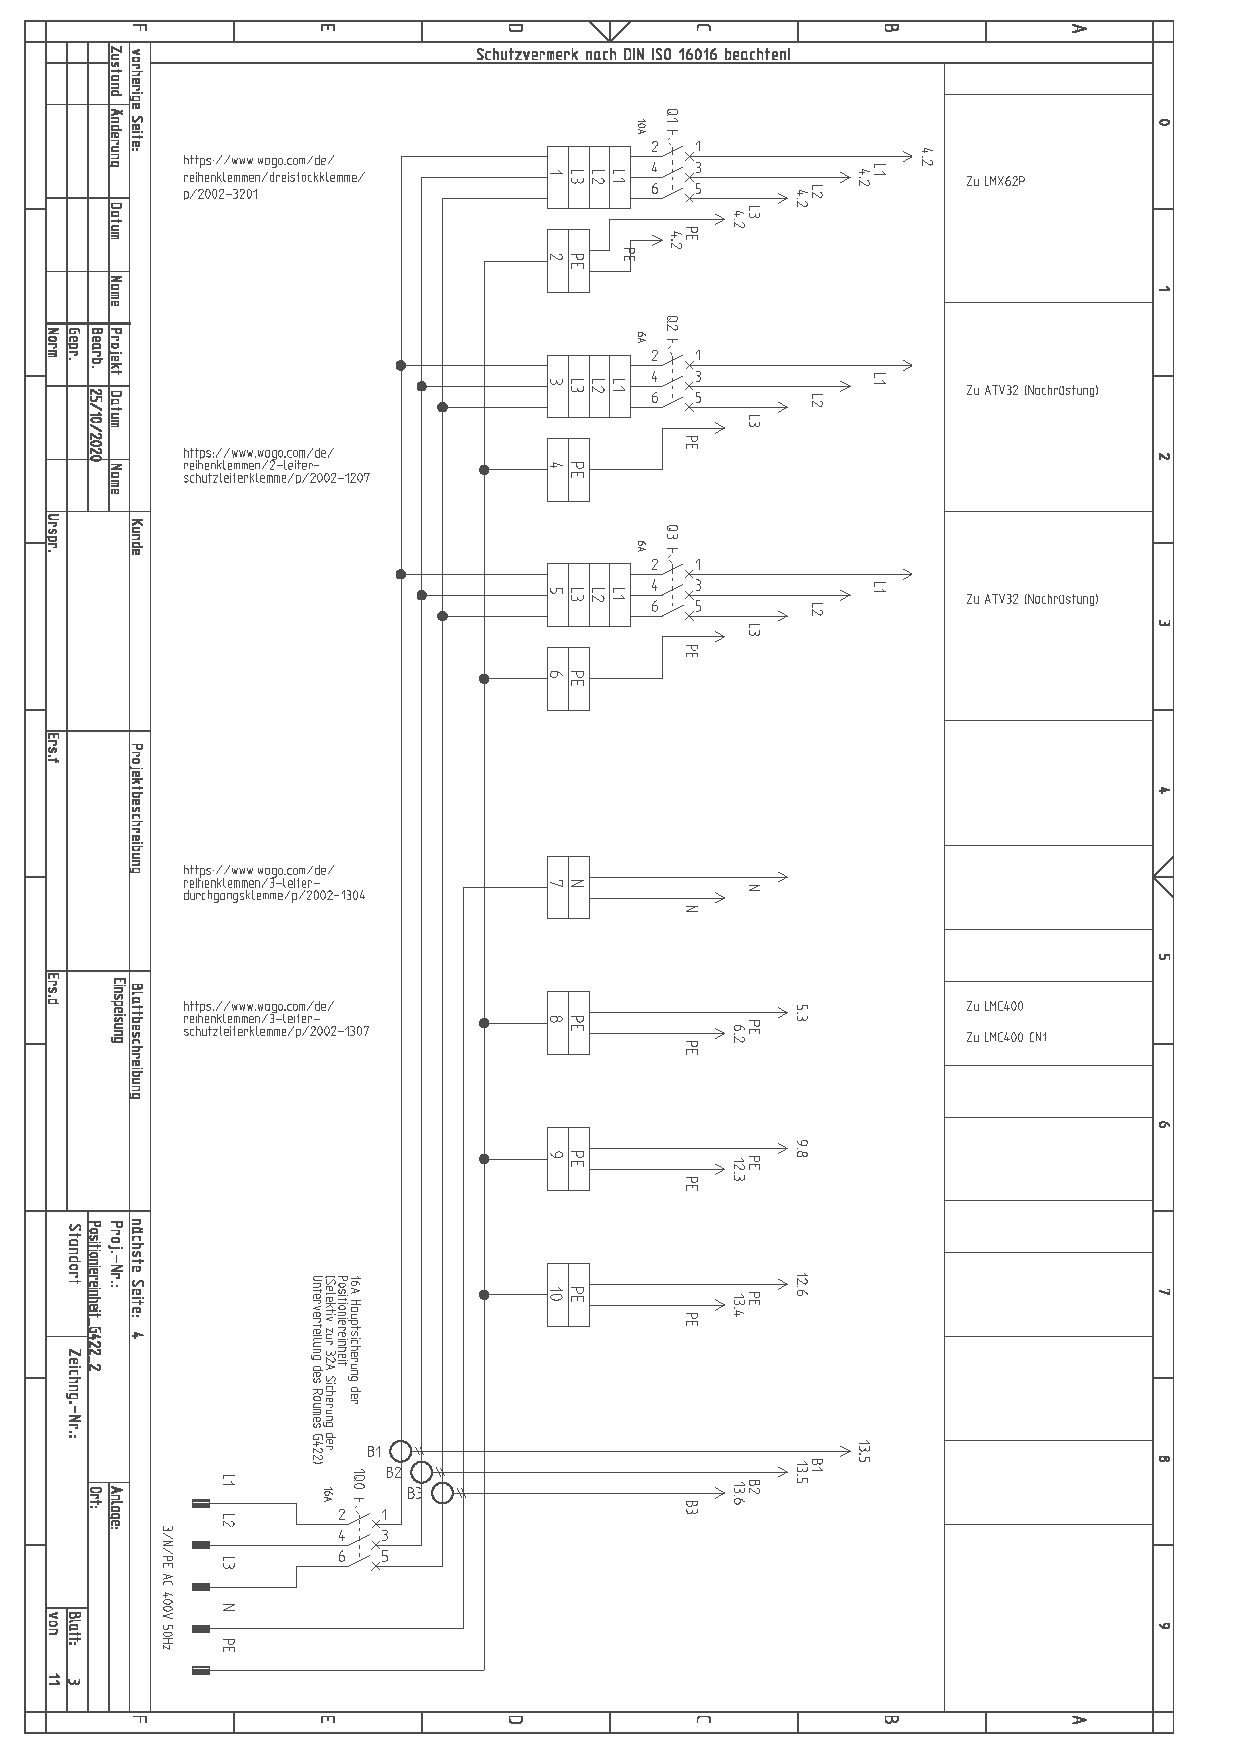
\includepdf{Images/slp3.pdf}
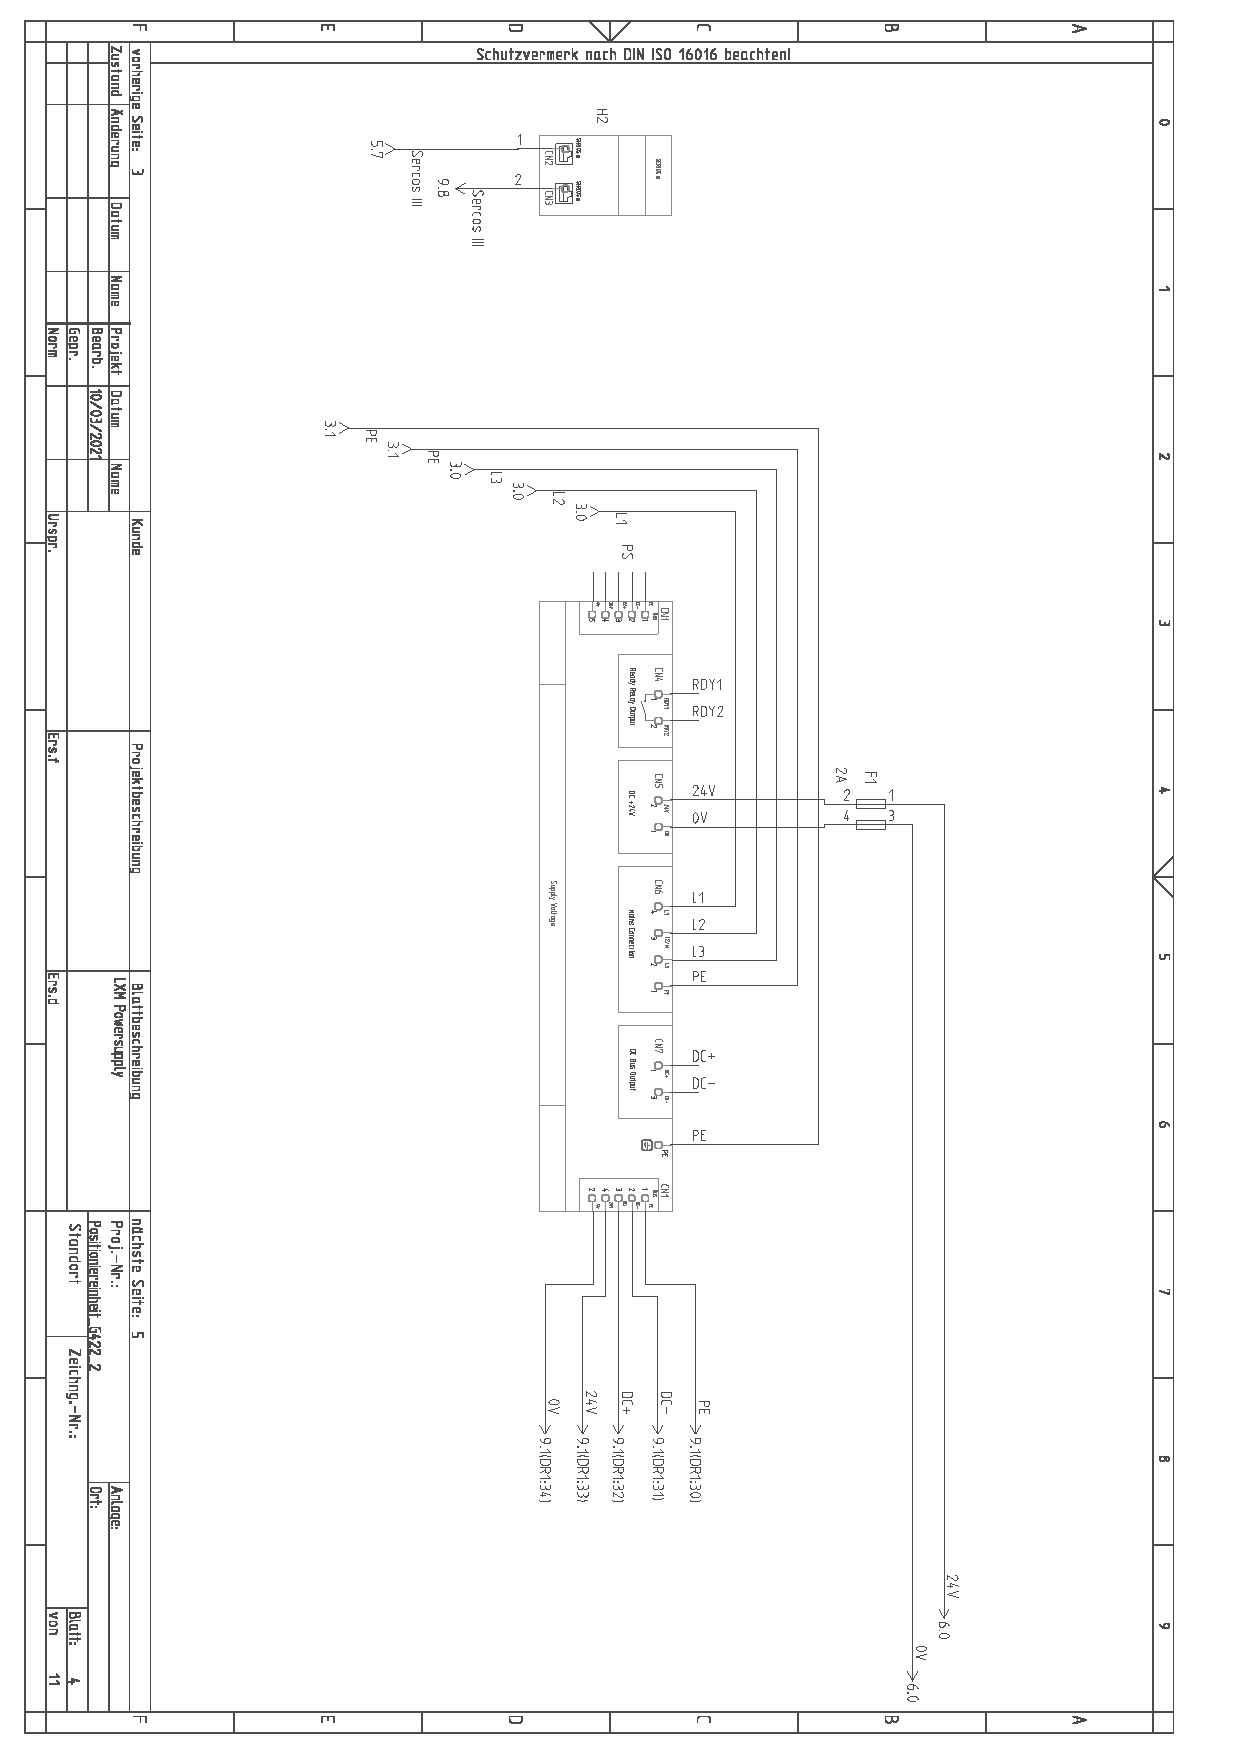
\includepdf{Images/slp4.pdf}
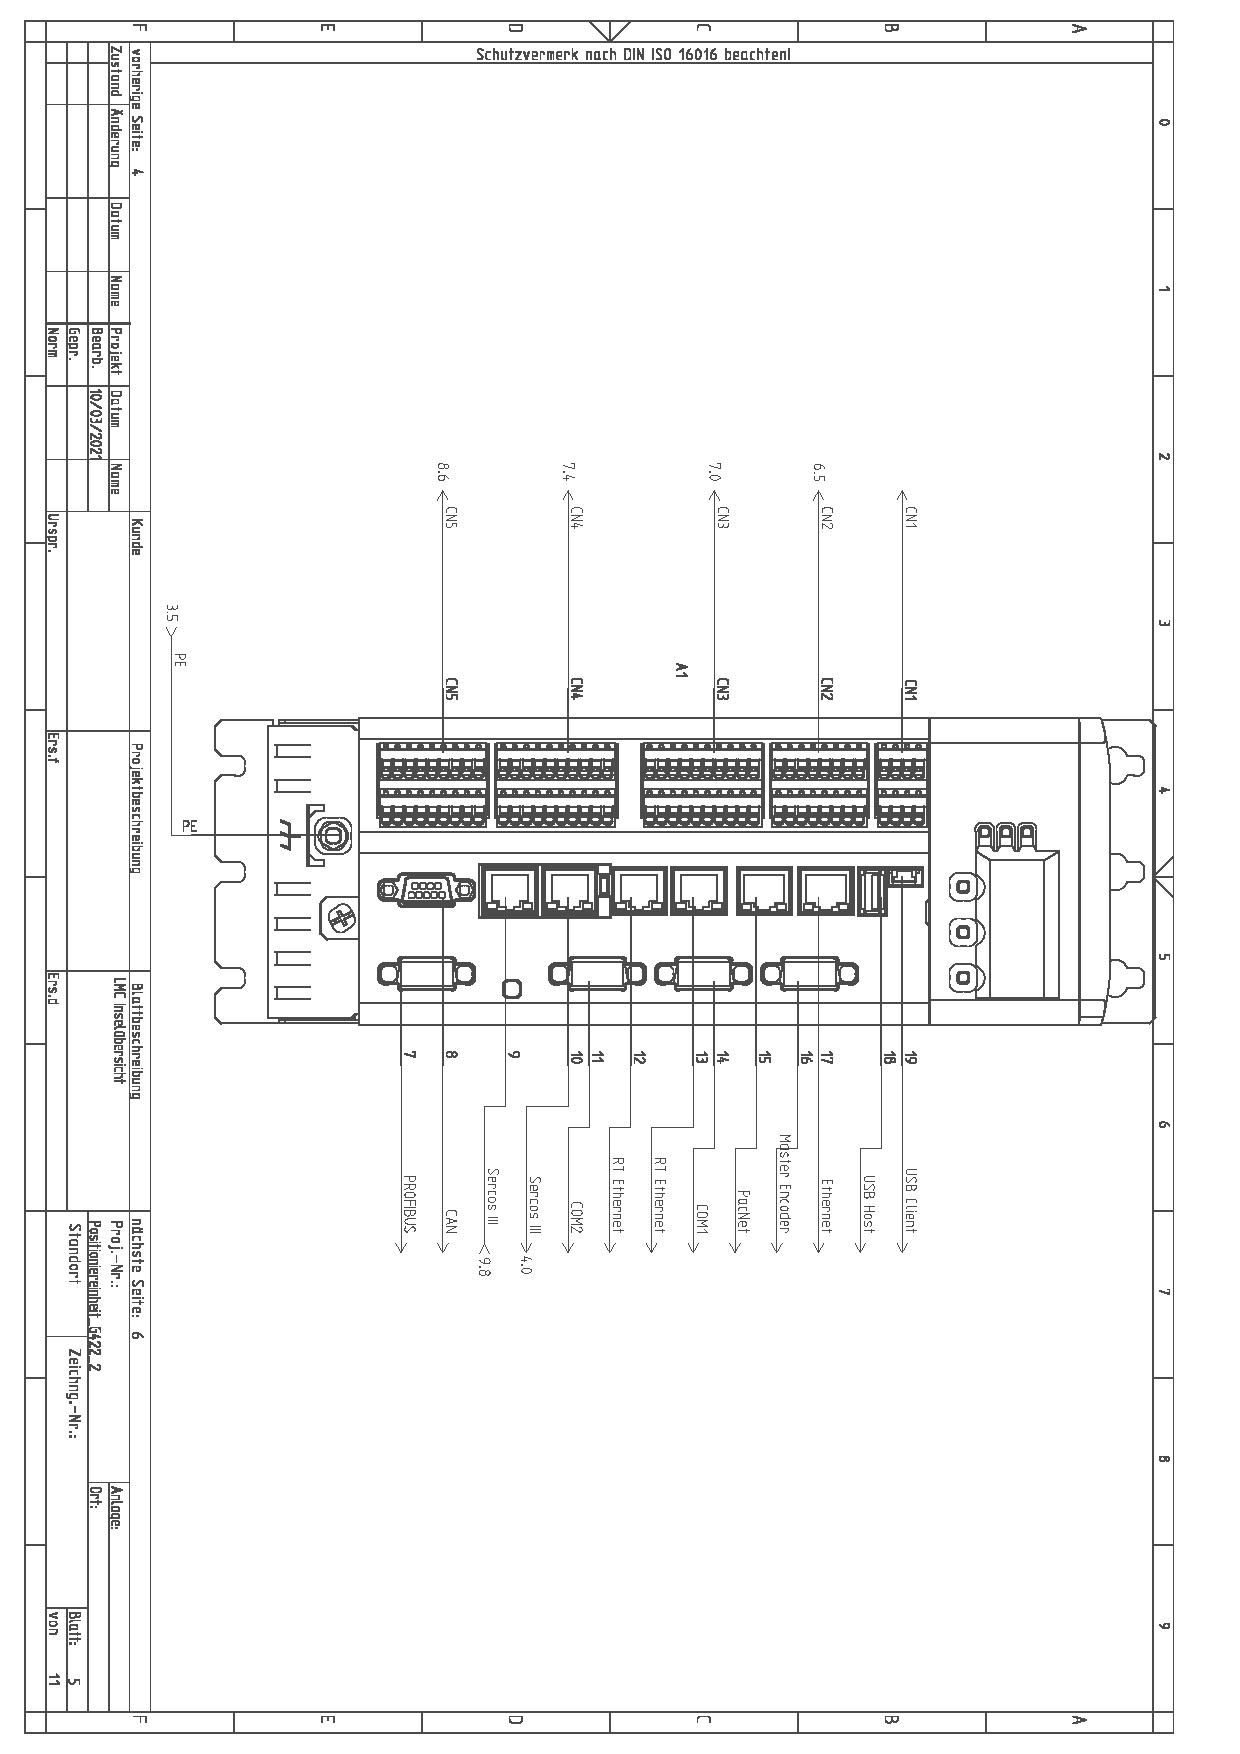
\includepdf{Images/slp5.pdf}
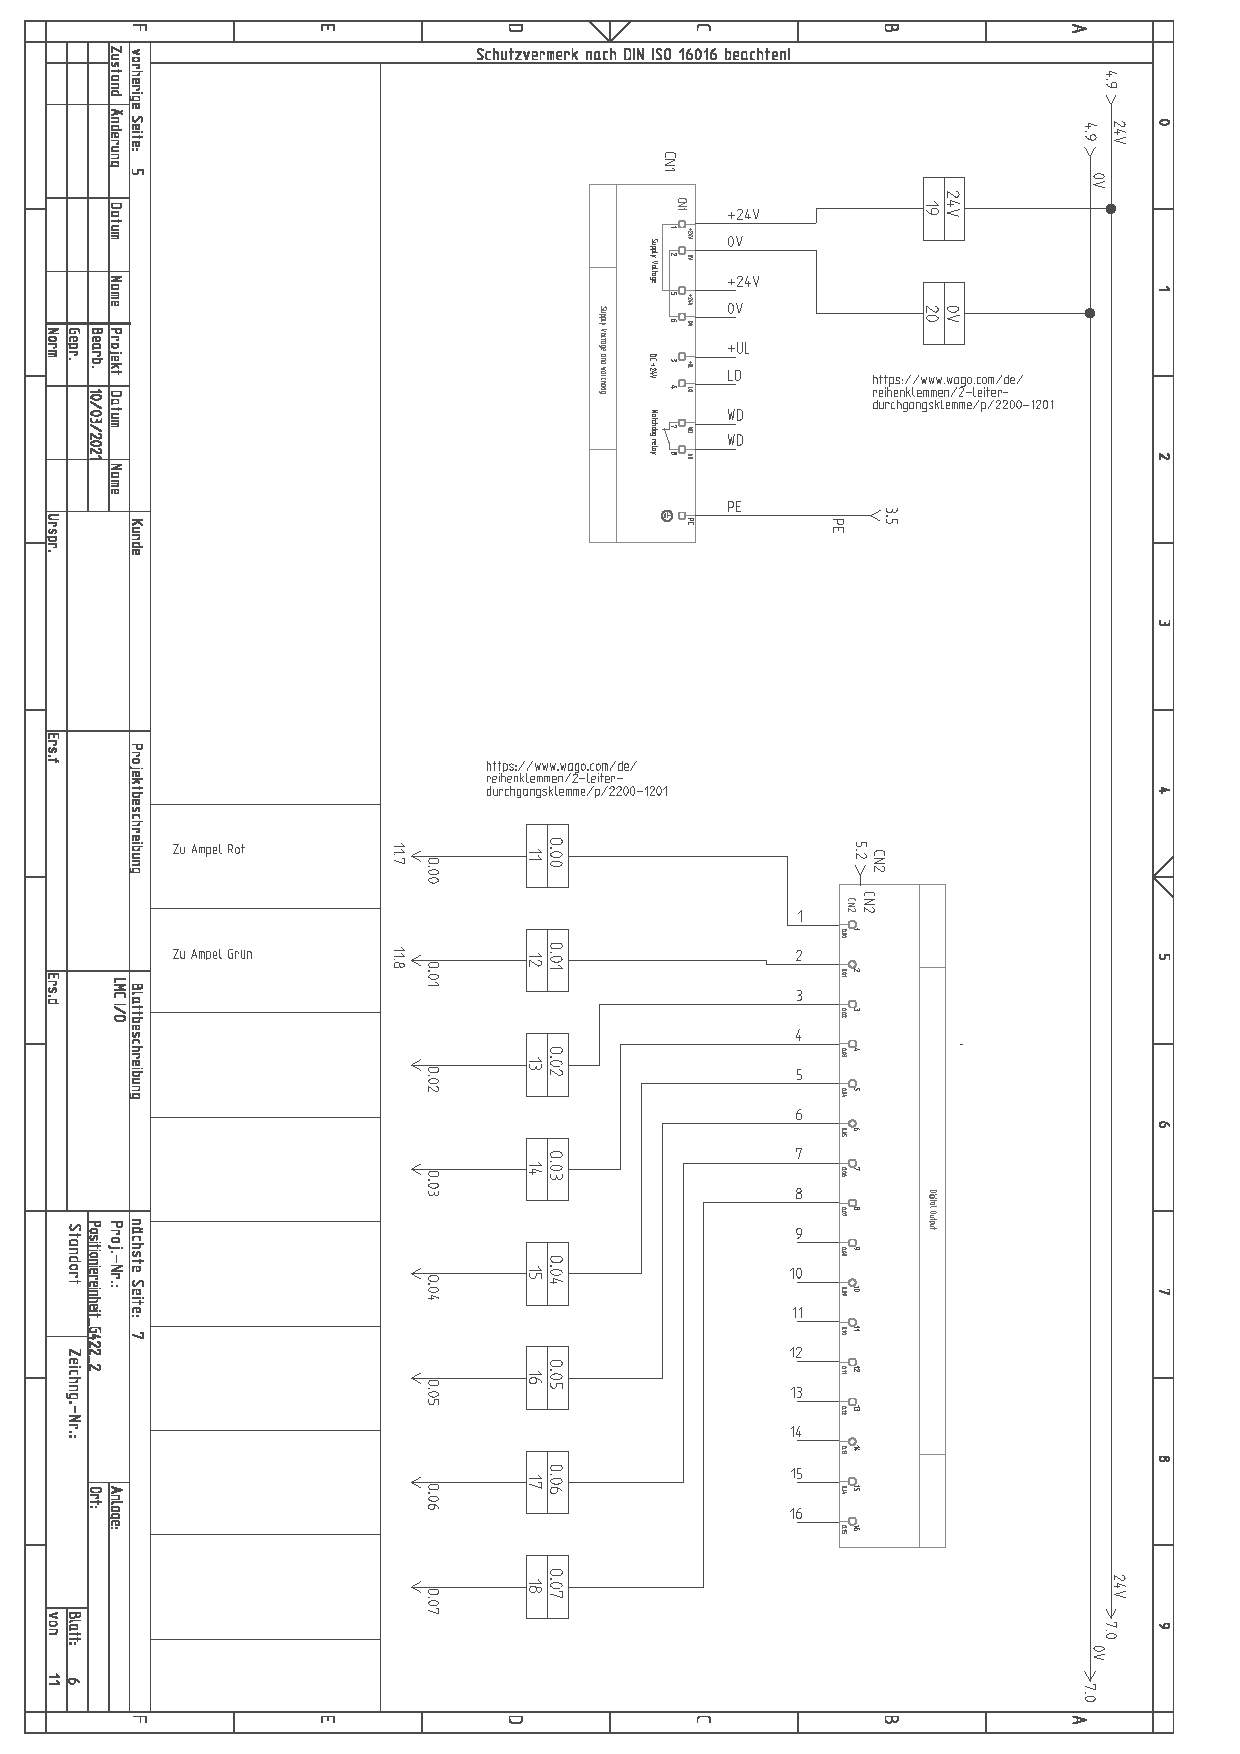
\includepdf{Images/slp6.pdf}
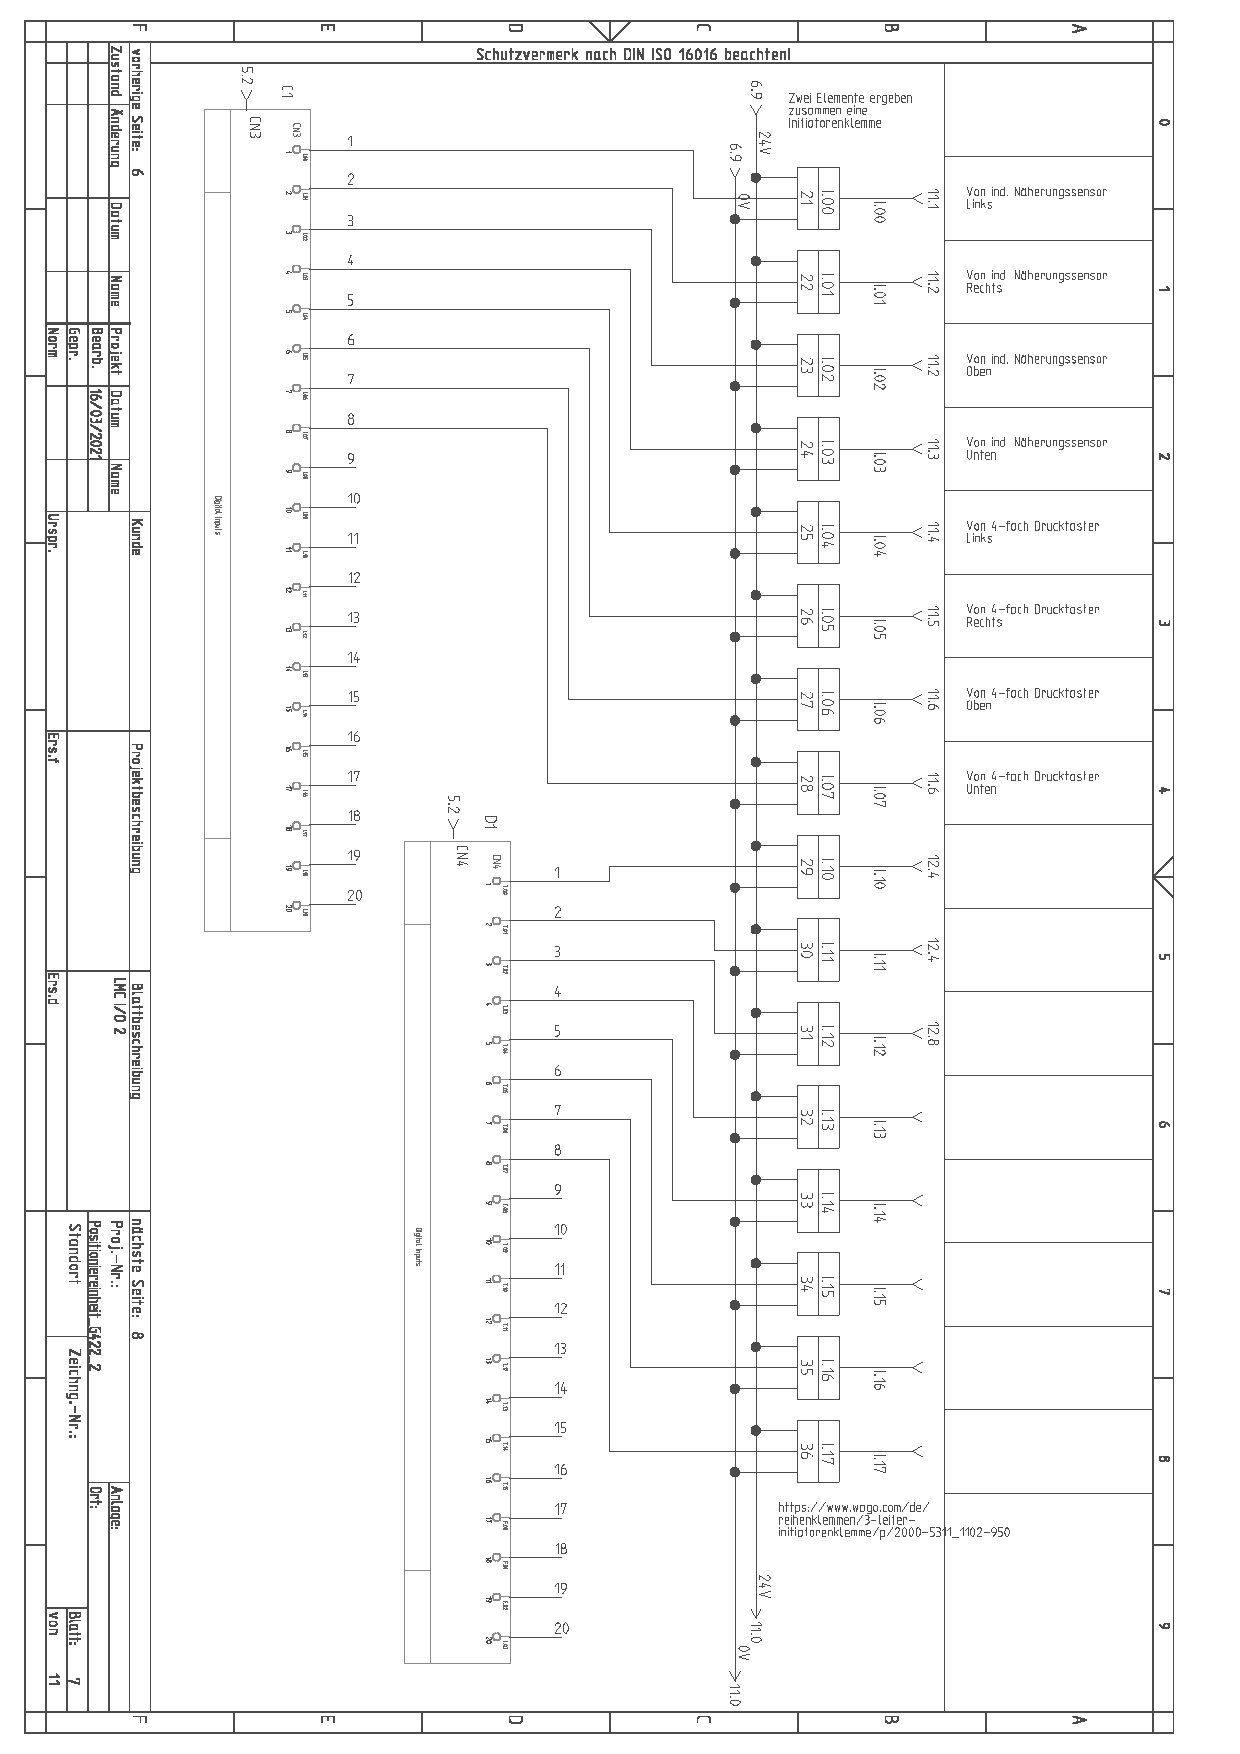
\includepdf{Images/slp7.pdf}
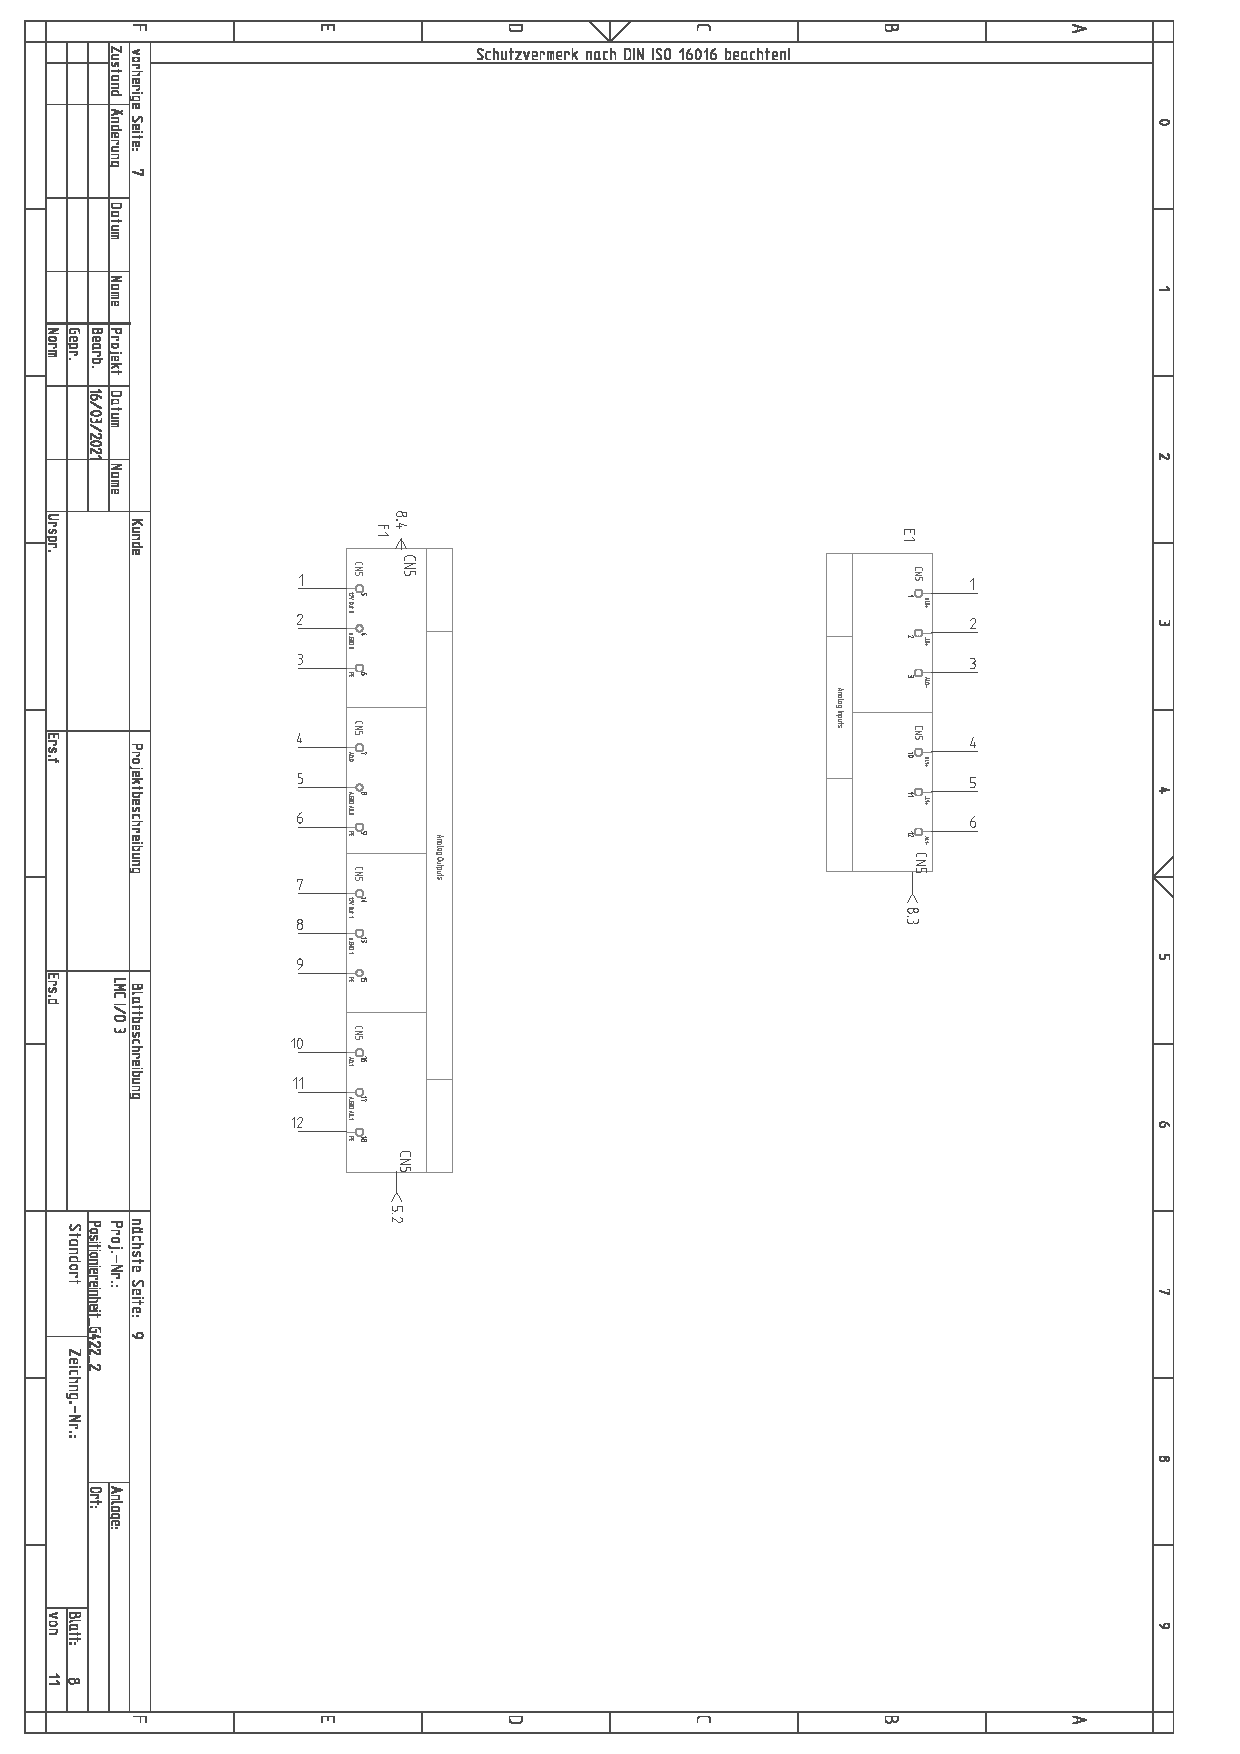
\includepdf{Images/slp8.pdf}
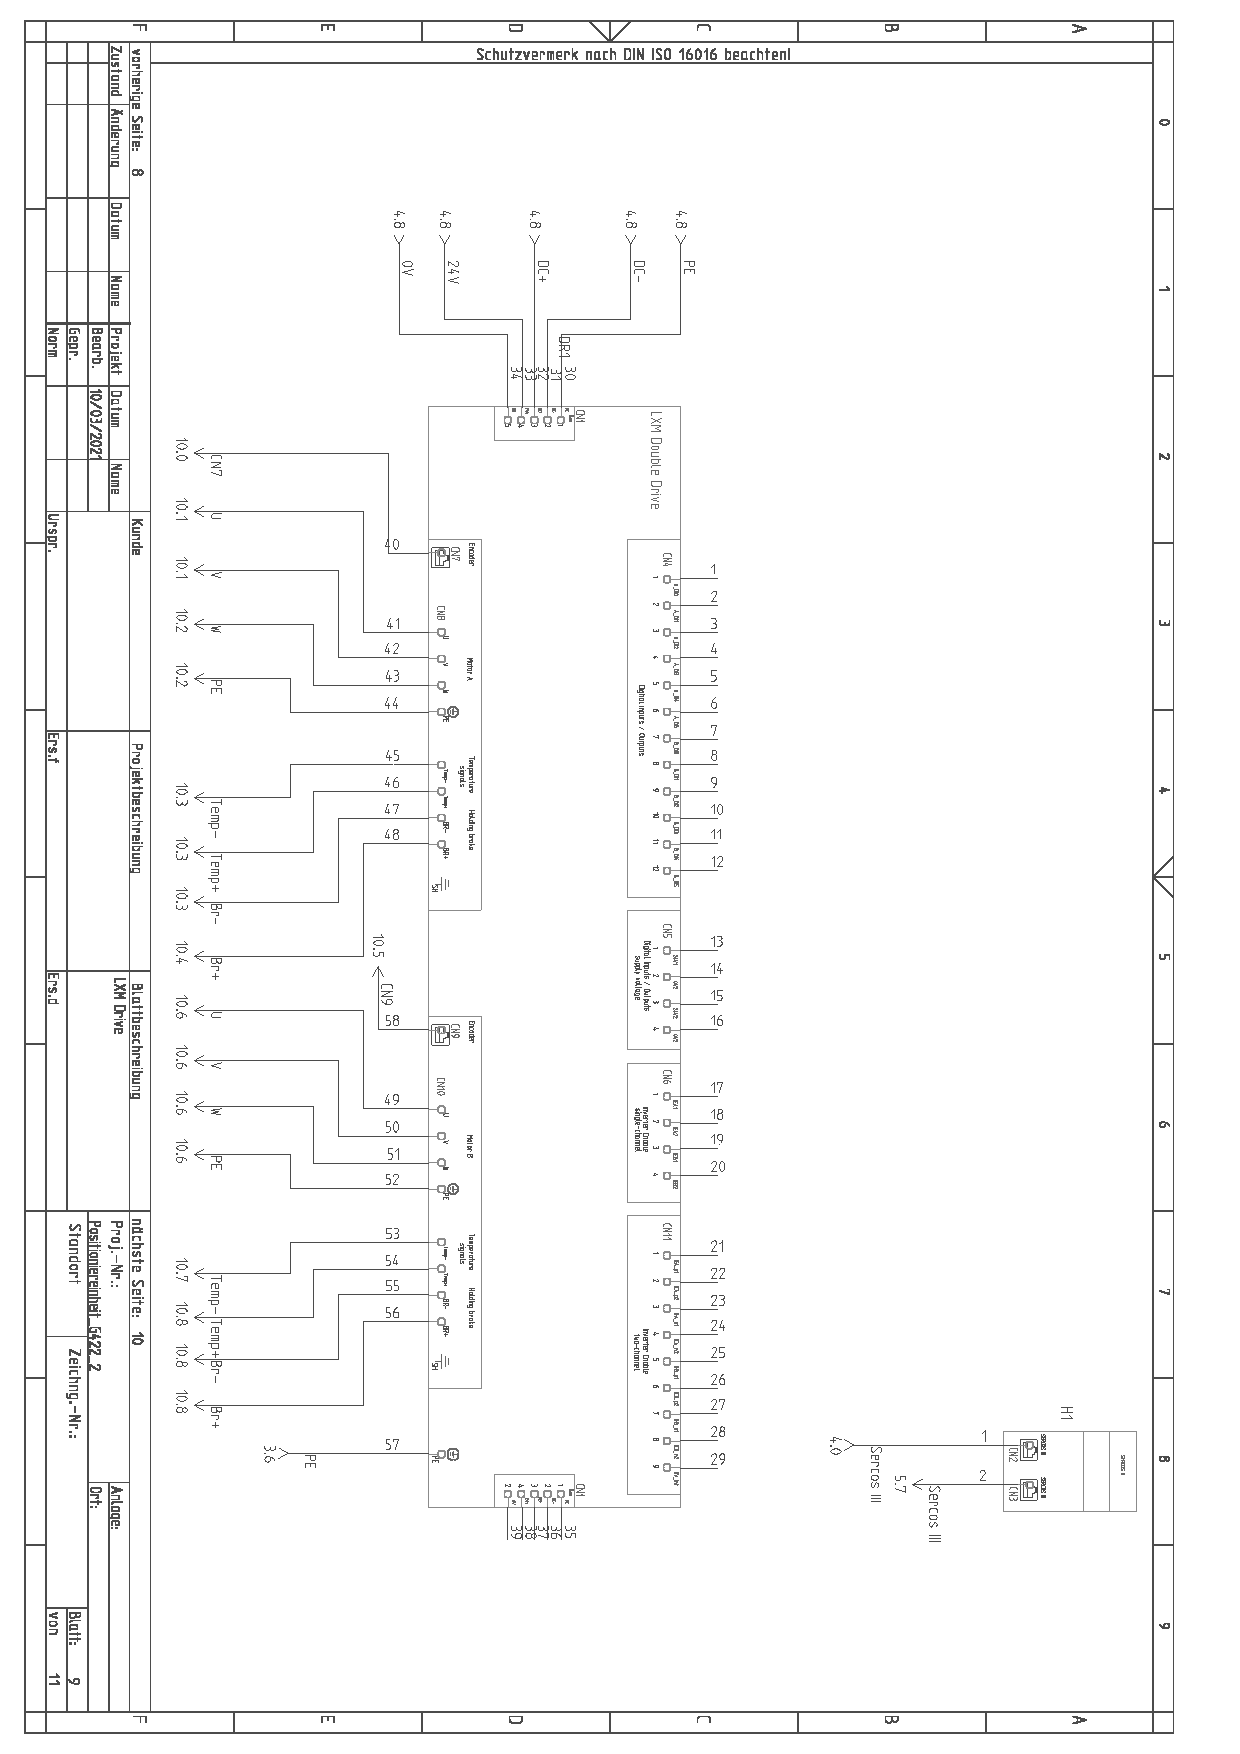
\includepdf{Images/slp9.pdf}
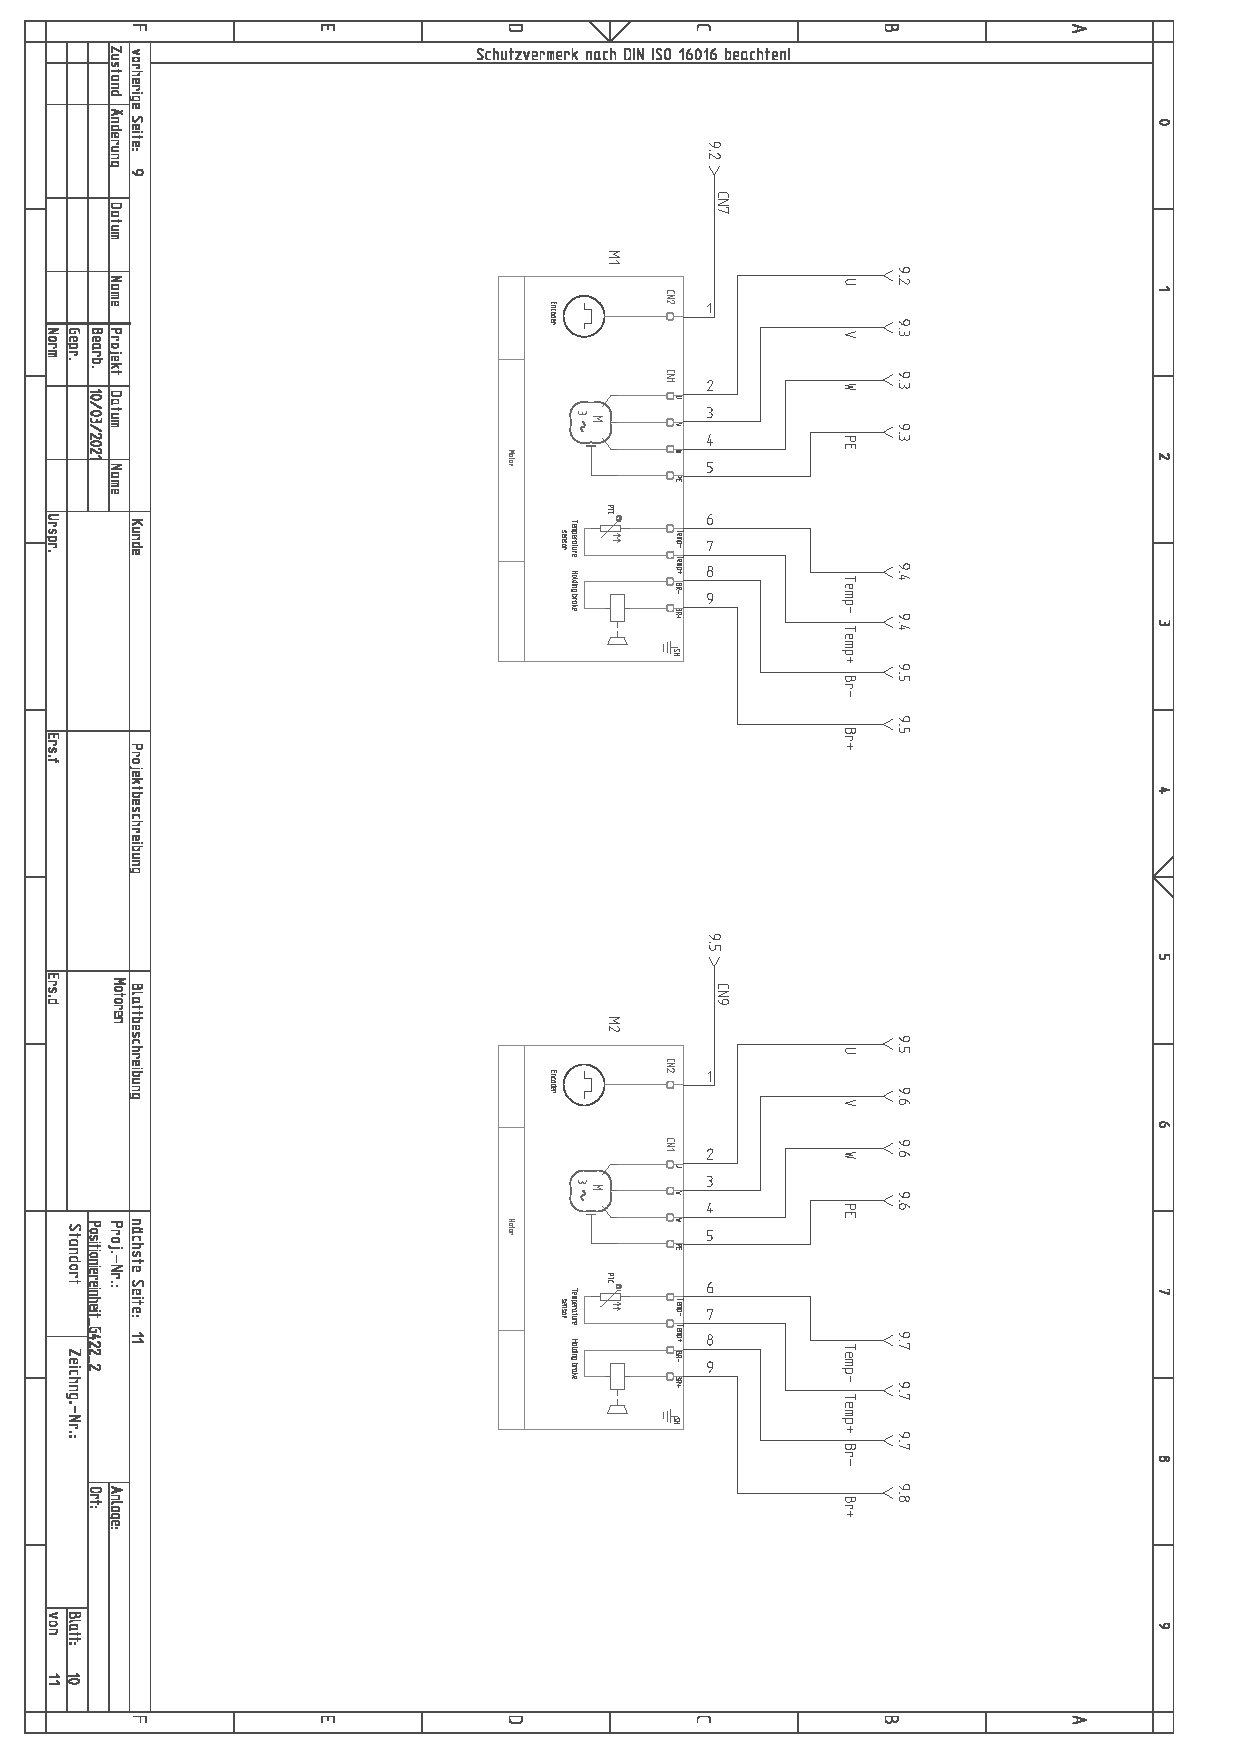
\includepdf{Images/slp10.pdf}
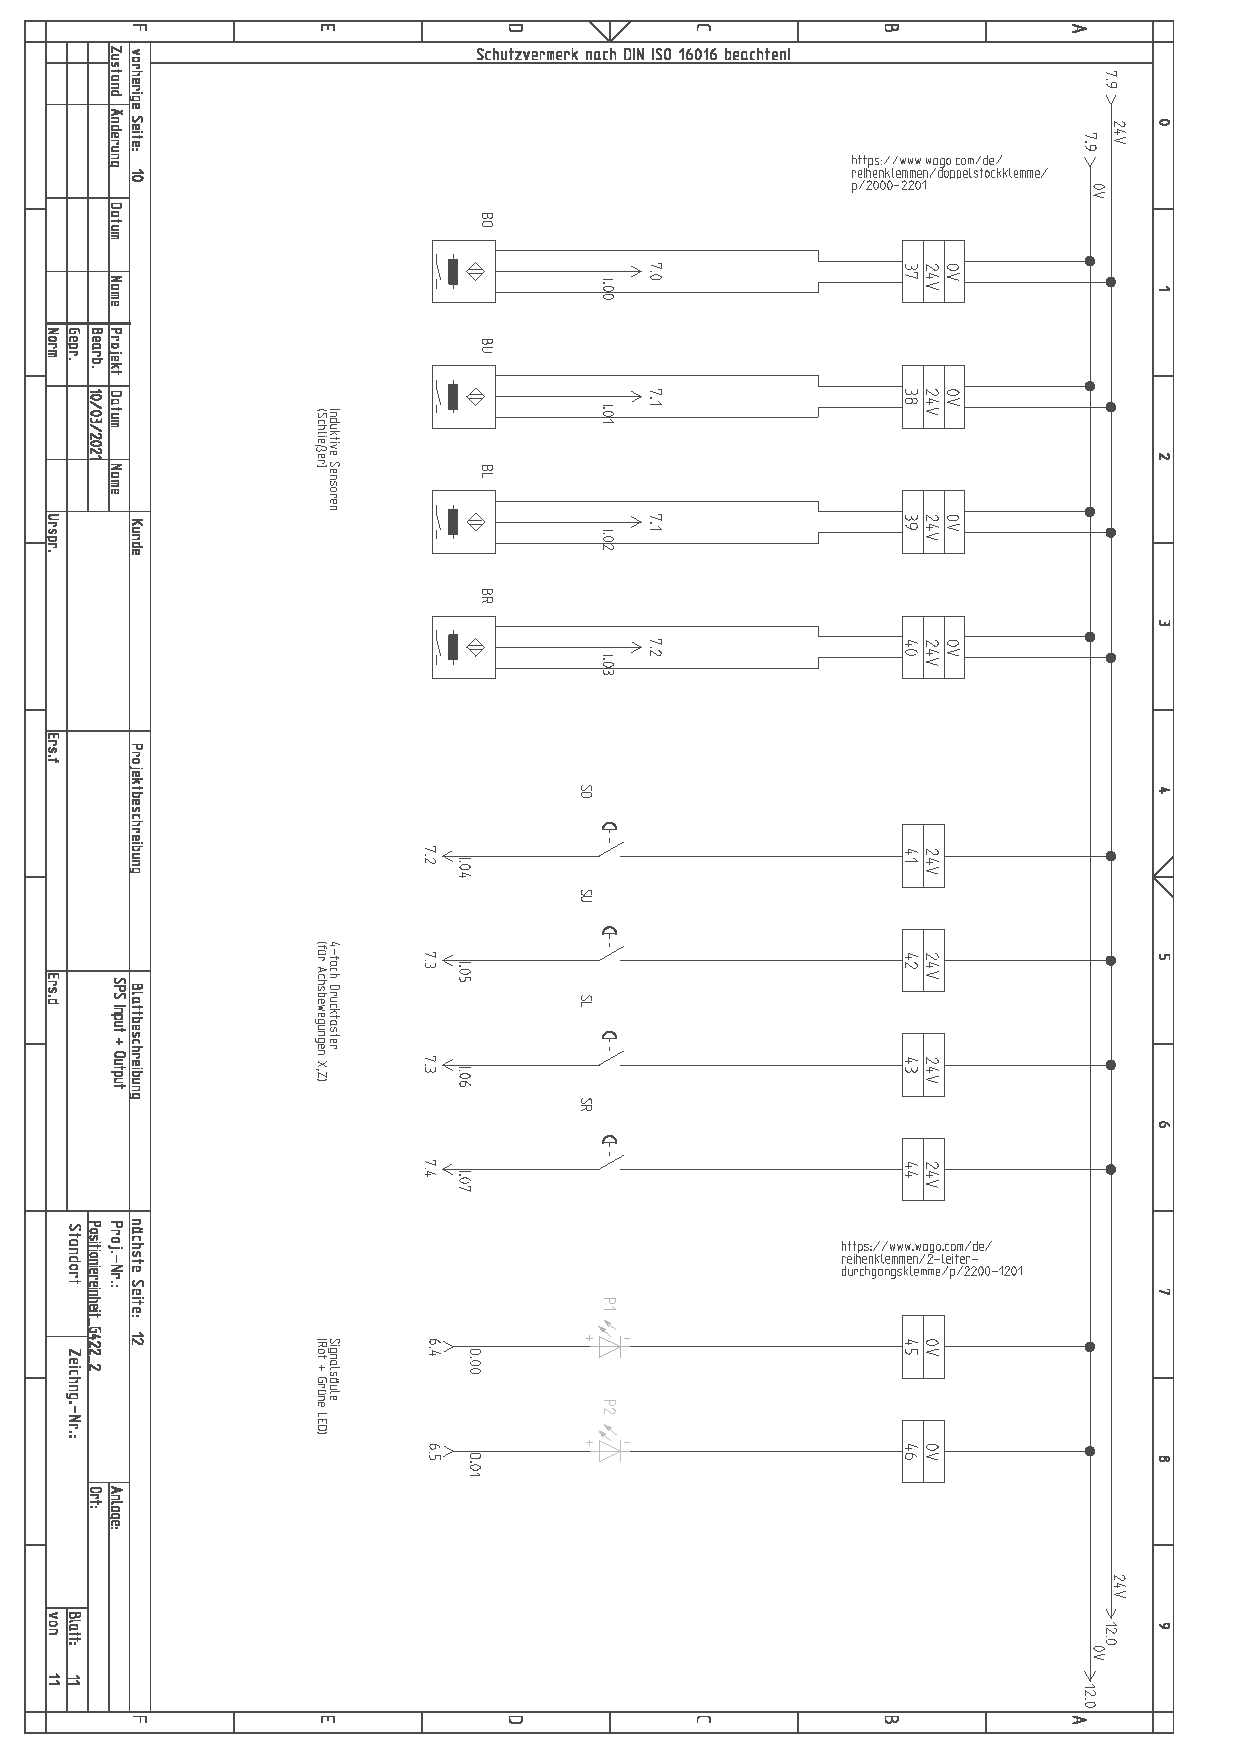
\includepdf{Images/slp11.pdf}
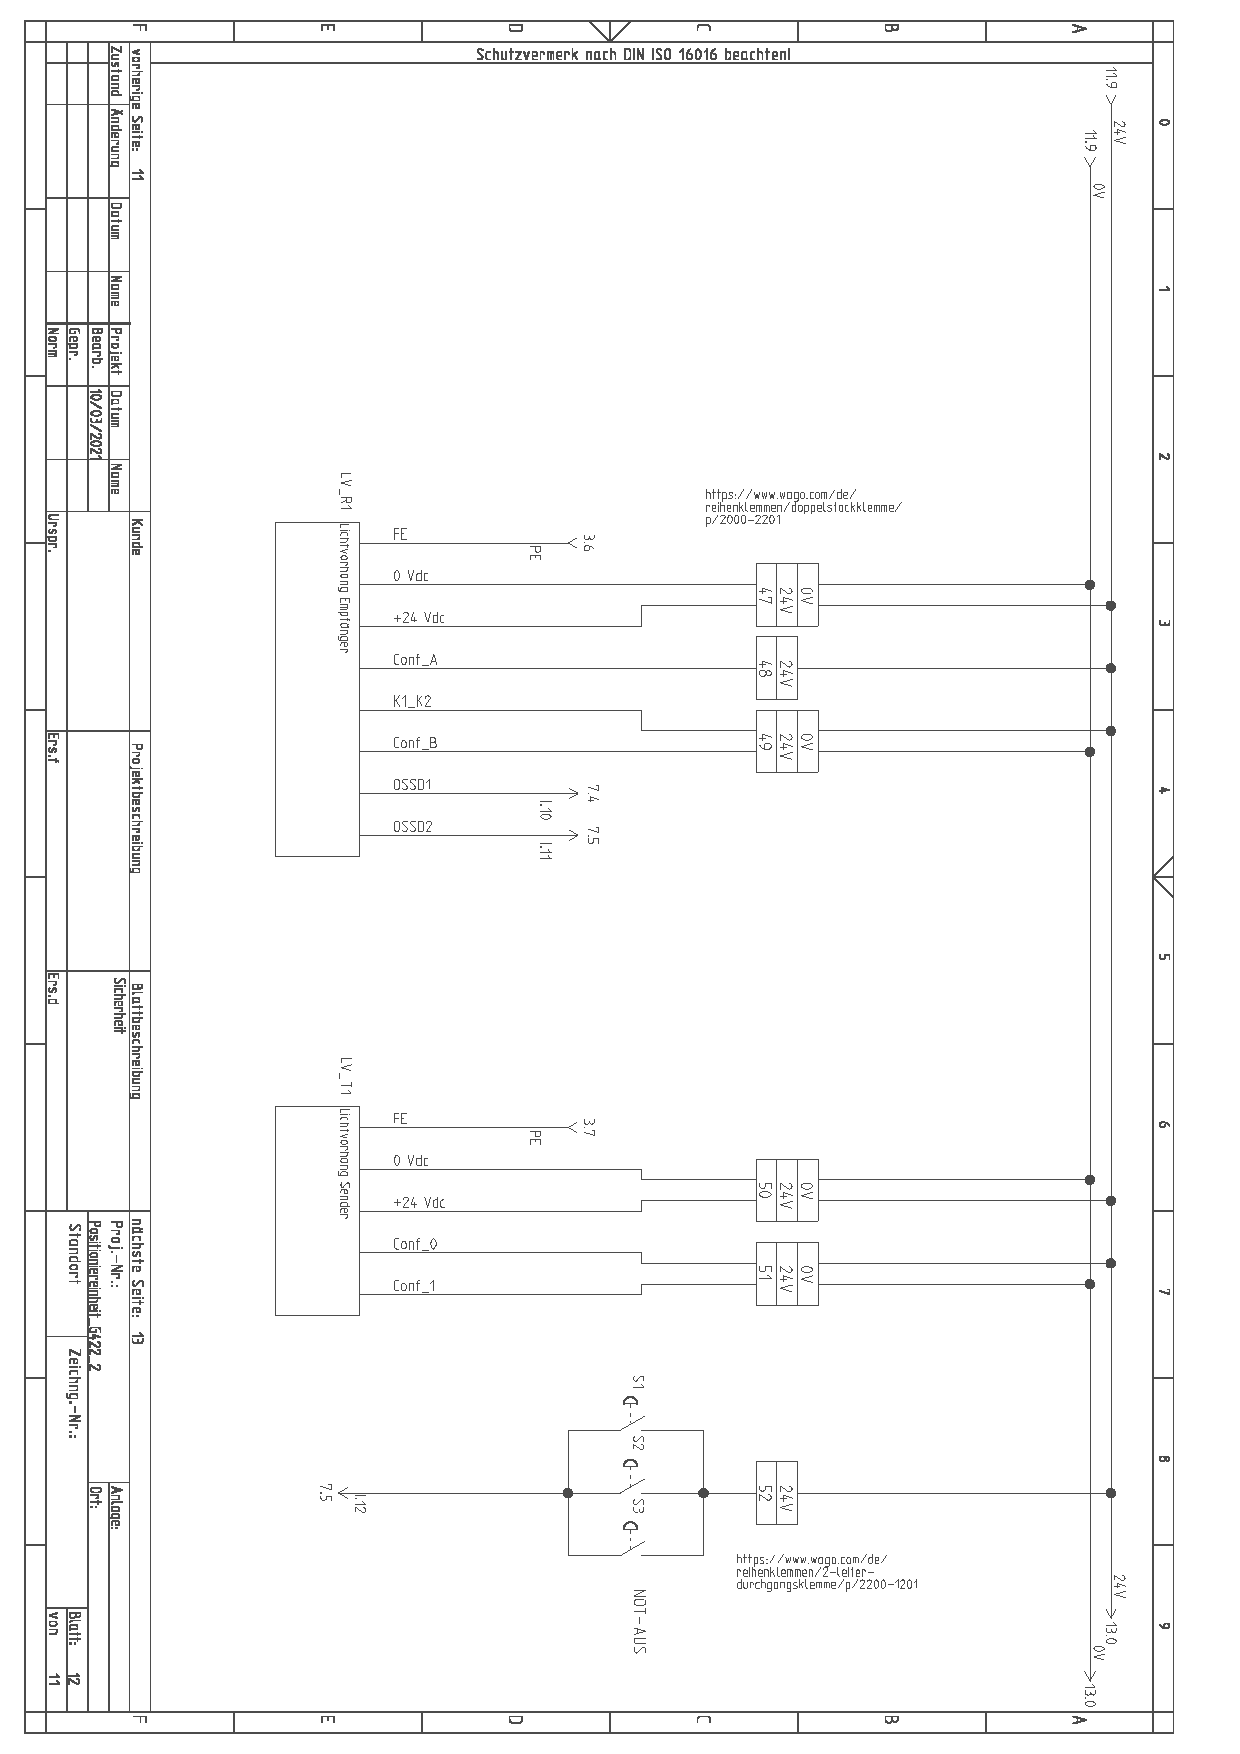
\includepdf{Images/slp12.pdf}
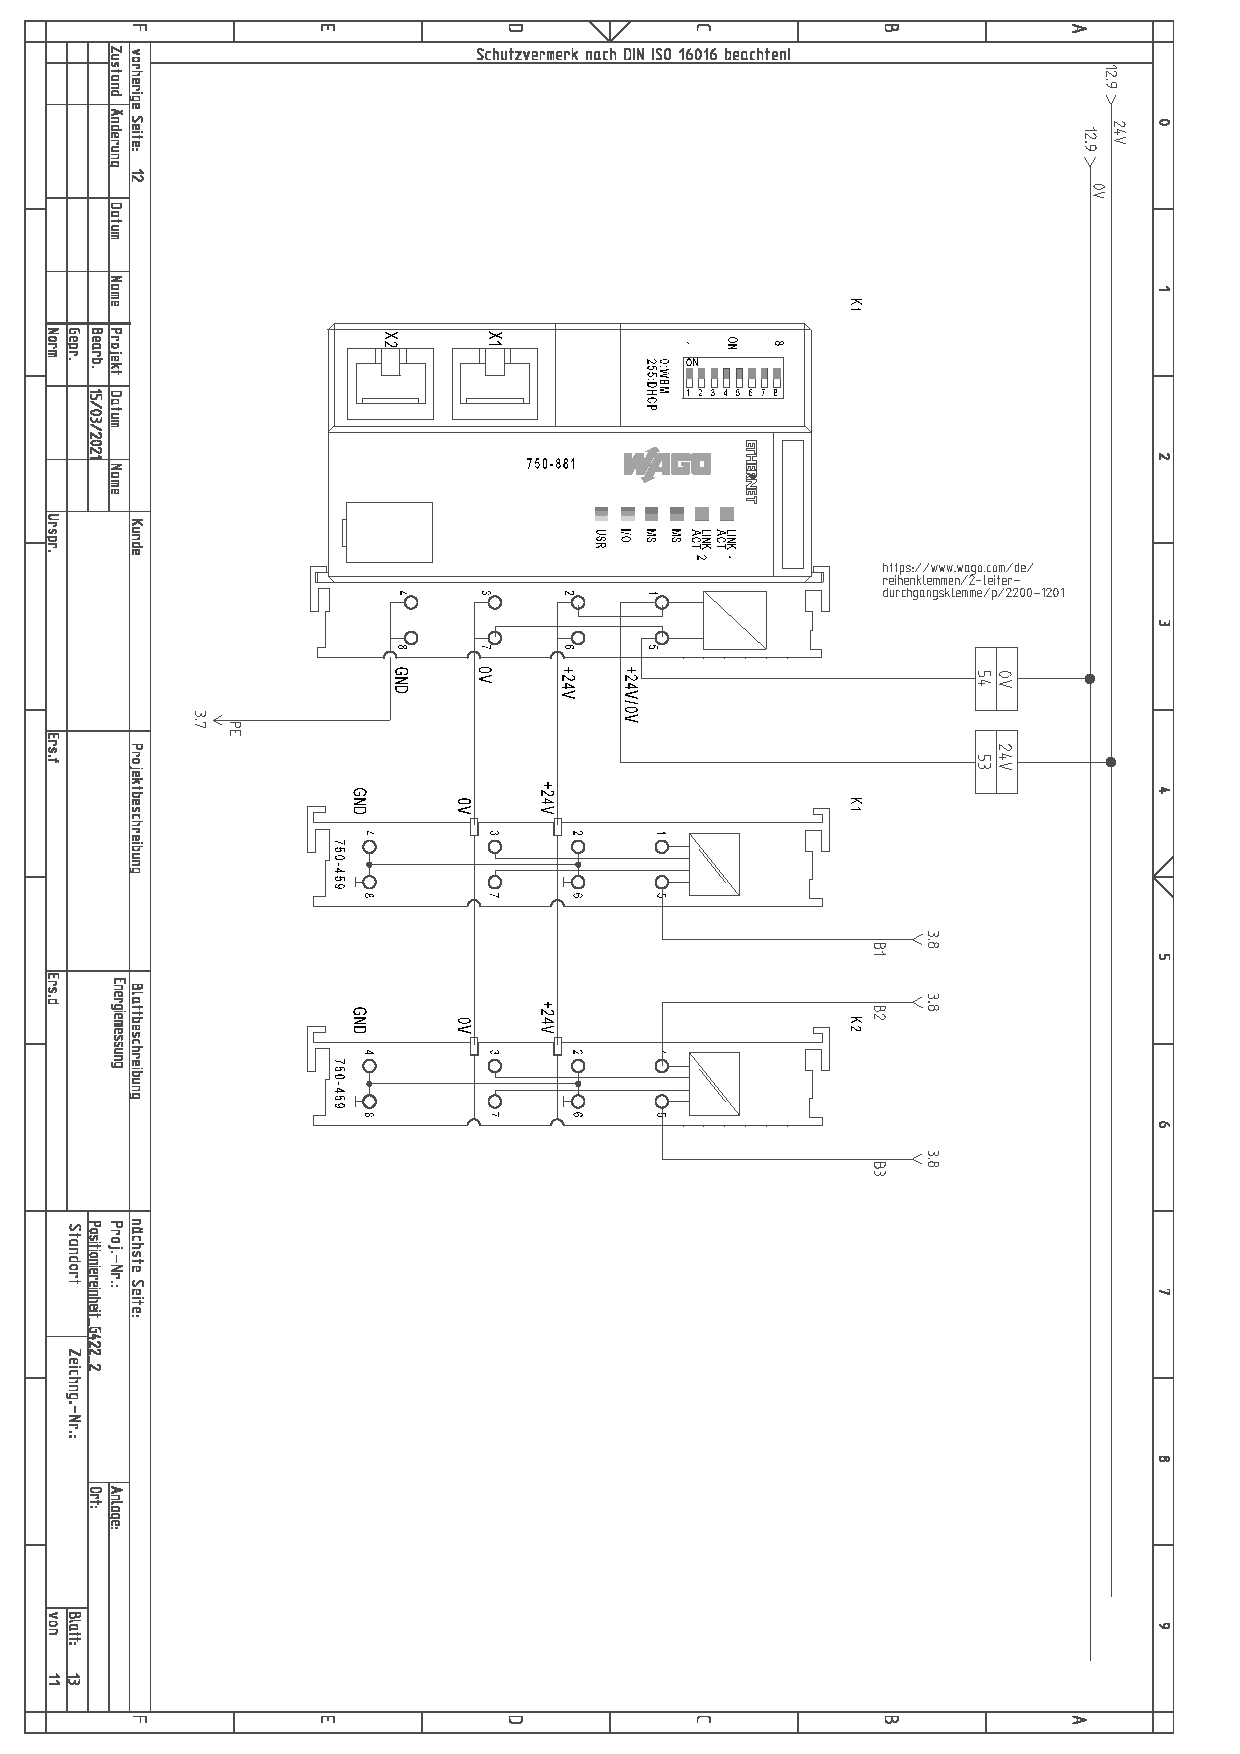
\includepdf{Images/slp13.pdf}

\end{document}